\subsubsection{Merge Sort}

Figure \ref{fig:net_merge_sort} illustrates the time it takes for each language, run in the .NET environment, to sort one million randomly generated positive integers in ascending order.

\begin{figure}[h]
	\centering
	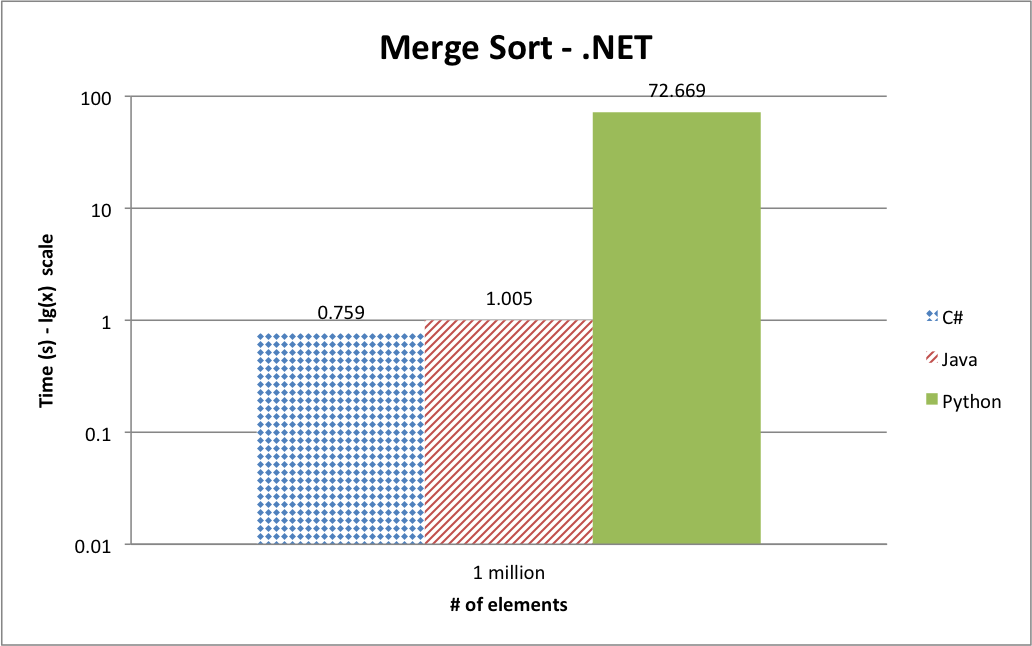
\includegraphics[width=1.0\linewidth]{chapters/new_media/MergeSortNet.png}
	\caption{This test is run in the .NET environment and uses the Merge sort algorithm to sort one million elements in ascending order. A lower value is better. Note that the vertical axis is base 10 logarithmic. C\# is the fastest with 0.759 seconds. Java comes in second with 0.967 seconds. Python is the slowest with 71.663 seconds.}
	\label{fig:net_merge_sort}
\end{figure}

Figure \ref{fig:net_merge_sort_memory} illustrates the amount of MB of memory used when running the merge sort algorithm in the .NET environment by the different languages. C\# and Java are almost equal while Python uses more memory.

\begin{figure}[h]
	\centering
	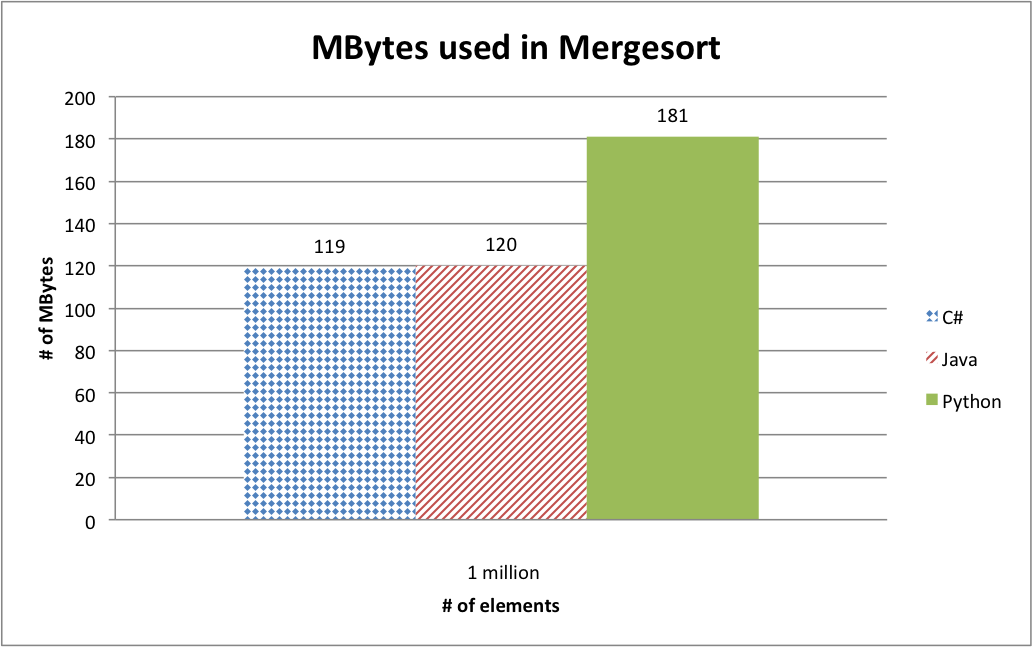
\includegraphics[width=1.0\linewidth]{chapters/new_media/MBytesMergesort.png}
	\caption{This test is run in the .NET environment and uses the Merge sort algorithm to sort one million elements in ascending order. A lower value is better. C\# and Java perform equally with 119MB and 120MB of memory used. Python performs the worst with 181MB of memory used. }
	\label{fig:net_merge_sort_memory}
\end{figure}

Figure \ref{fig:net_merge_sort_processor} illustrates the percentage of the processor used when running the merge sort algorithm in the .NET environment by the different languages.

\begin{figure}[h]
	\centering
	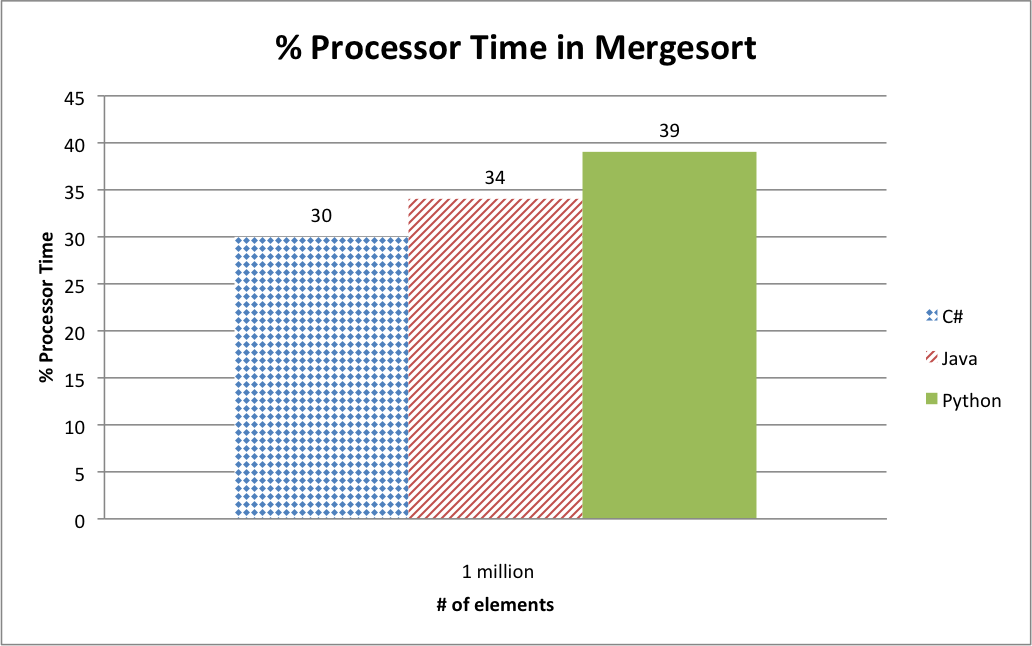
\includegraphics[width=1.0\linewidth]{chapters/new_media/ProcessorTime.png}
	\caption{This test is run in the .NET environment and uses the Merge sort algorithm to sort one million elements in ascending order. A lower value is better. C\# performs the best with 30\% processor usage, Java is a close second with 34\% and Python performs the worst with 39\%. }
	\label{fig:net_merge_sort_processor}
\end{figure}
